% Very simple template for lab reports. Most common packages are already included.
\documentclass[a4paper, 11pt]{article}
\usepackage[utf8]{inputenc} % Change according your file encoding
\usepackage{graphicx}
\usepackage{url}
\usepackage{fourier}
\usepackage{listings}
\lstset{
  morekeywords={abort,abs,accept,access,all,and,array,at,begin,body,
      case,constant,declare,delay,delta,digits,do,else,elsif,end,entry,
      exception,exit,for,function,generic,goto,if,in,is,limited,loop,
      mod,new,not,null,of,or,others,out,package,pragma,private,
      procedure,raise,range,record,rem,renames,return,reverse,select,
      separate,subtype,task,terminate,then,type,use,when,while,with,
      xor,abstract,aliased,protected,requeue,tagged,until,public,static,void},
  sensitive=f,
  morecomment=[l]\#,
  morestring=[d]",
  showstringspaces=false,
  basicstyle=\small\ttfamily,
  keywordstyle=\bf\small,
  commentstyle=\itshape,
  stringstyle=\sf,
  extendedchars=true,
  columns=[c]fixed,
  numbers = left,
  numberstyle=\tiny,
  stepnumber=2,
  numbersep=5pt,
  framexleftmargin=5mm,
  language=R,
  frame=shadowbox
}

% CI-DESSOUS: conversion des caractères accentués UTF-8 
% en caractères TeX dans les listings...
\lstset{
  literate=%
  {À}{{\`A}}1 {Â}{{\^A}}1 {Ç}{{\c{C}}}1%
  {à}{{\`a}}1 {â}{{\^a}}1 {ç}{{\c{c}}}1%
  {É}{{\'E}}1 {È}{{\`E}}1 {Ê}{{\^E}}1 {Ë}{{\"E}}1% 
  {é}{{\'e}}1 {è}{{\`e}}1 {ê}{{\^e}}1 {ë}{{\"e}}1%
  {Ï}{{\"I}}1 {Î}{{\^I}}1 {Ô}{{\^O}}1%
  {ï}{{\"i}}1 {î}{{\^i}}1 {ô}{{\^o}}1%
  {Ù}{{\`U}}1 {Û}{{\^U}}1 {Ü}{{\"U}}1%
  {ù}{{\`u}}1 {û}{{\^u}}1 {ü}{{\"u}}1%
}
%opening
\title{Report 3: Loggy, a logical time logger}
\author{Simon Cathébras}
\date{\today{}}

\begin{document}
\maketitle
\section{Introduction}

\subsection{Context}
During this assignment, we have manipulated logical time, and more specifically Lamport's clock.This assignment has highlighted that, more than the time itself, the ordering of events is a critical issue in distributed systems. Moreover, measuring precisely the time, is something very difficult to do in computer science. And thus, trying to synchronize several component of a distributed system with physical time, is impossible to do in real life. That's why Lamport's logical time only relies on event's ordering. But, even if this concept seems easy to understand, implementing it can be a little bit tricky. \\

\subsection{What have been realised}
We implemented the Lamport's clock mechanism for the logger. The worker are keeping trace of their own state, and this state is updated each time a message is received. The Logger keeps a queue of message "not safe to print yet", and a list containing each workers and their respective states. A message is printed out of the queue when his \lstinline!TimeStamp! is less than the minimum of worker's state.
The output seems correct. Unfortunately, we could only verify this correction ourselves, instead of writing a program to do so.

\section{Main problems and solutions}
\paragraph{Spot wrong ordering}
Our first main problem was to spot wrong ordering in the first implementation. We solved this when we realised that when a message was displayed as \lstinline!received! before be displayed as \lstinline!sent!, then, there is a problem somewhere...

\paragraph{Lamport Clock}
Implementing the change of states inside each processes was not really a problem. As a matter of fact, the problem was, as the logger: "When can I write a message safely ?". We first solved this in realising that a message can be displayed when we are sure to not receive a message with an older \lstinline!TimeStamp!. Then, we needed a way to be sure that for a given \lstinline!TimeStamp!, we would not receive a message with an inferior \lstinline!TimeStamp!. We solved this with the following:
\begin{itemize}
\item The logger keeps tracks of the states of each process with a list of t-uples: \lstinline!{ProcessName, Time}!
\item The logger has a \lstinline!CurrentStamp!.
\item Whenever the logger receives a message, the state list of all processes is updated. Then it checks if the message's \lstinline!TimeStamp! is bellow or equal to \lstinline!CurrentStamp!. If so, the message is displayed right now. If not, the message is stored in the \lstinline!Queue! and we are looking if the minimum Time of the state list of processes is greater than \lstinline!CurrentStamp!. If so, we update the stamp and we flush the \lstinline!Queue! of all messages with a \lstinline!Stamp! less than the new \lstinline!CurrentStamp!. Note, that before we drain the Queue, it MUST be ordered.
\end{itemize}

\paragraph{Efficiency and reliability}
After we found out how to implement the Lamport's ordering, we wondered if our solution was correct concerning efficiency and resources consumption. That's why we implemented a function to check the size of the list during the execution of the scenario.
Here are the results we observed.\\

\begin{center}
\begin{tabular}{|c|c|c|c|c|}
\hline 
Number of Processes & 5 & 10 & 15 & 20 \\ 
\hline 
Maximum size of the queue & 20 & 56 & 129 & 193 \\ 
\hline 
\end{tabular} 
\end{center}


It appears that this implementation is very greedy in resources when there is an increase of the number of clients (See the graphic in Annexe). I look forward to discuss it during the seminar.

\section{Conclusion}
This assignment raised several issues about time management inside of distributed systems. The thing is, that implementing a Lamport's ordering is slightly more tricky than it appears at the first look.
\medskip

\section{Annexe}

\begin{figure}
  \begin{center}
    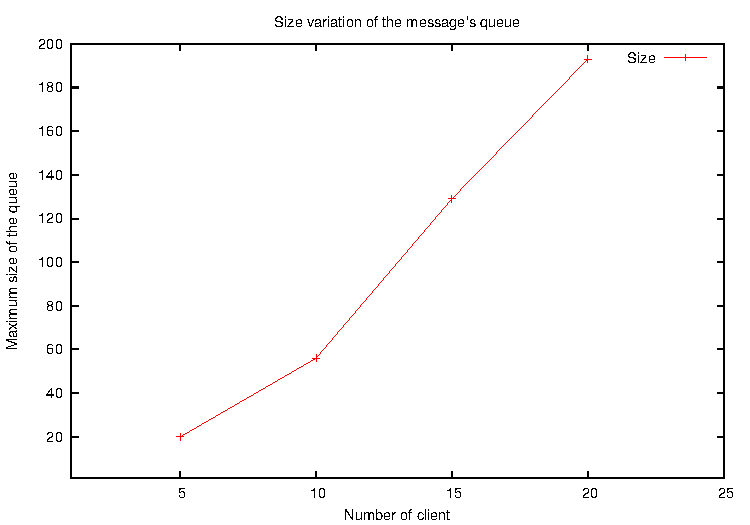
\includegraphics{size_queue}
    \caption{Length variation depending on number of workers}
    \label{fig:Size of Queue}
  \end{center}
\end{figure}

\end{document}